\documentclass[10pt,a4paper]{article}
\usepackage[utf8]{inputenc}
\usepackage[english]{babel}
\usepackage[square, numbers, sort&compress]{natbib}
\usepackage{graphicx}
\usepackage{float}
\usepackage{amsmath}
\usepackage{amsfonts}
\usepackage{amssymb}
%\usepackage{media9}
\usepackage{color}
\usepackage{fancyhdr}
\usepackage{lastpage}	
\usepackage{parskip}
\usepackage[scaled]{helvet}
\usepackage{blindtext}
\usepackage{sectsty}
\usepackage{multicol}
\usepackage{enumitem}
%\usepackage[svgnames]{xcolor}
\usepackage[labelfont={color=LibrelloColor,bf}, labelsep=period]{caption}
\renewcommand*{\familydefault}{\sfdefault}
\usepackage[left=1.75cm,right=1.75cm,top=1.75cm,bottom=3.75cm]{geometry}
\usepackage{titlesec}
\usepackage{svg}
\usepackage{flushend}
\PassOptionsToPackage{normalem}{ulem}
\usepackage{ulem}
	\providecolor{added}{rgb}{0,0,1}
	\providecolor{deleted}{rgb}{1,0,0}
	%% Change tracking with ulem
	\newcommand{\added}[1]{{\color{added}{}#1}}
	\newcommand{\deleted}[1]{{\color{deleted}\sout{#1}}}
\usepackage{setspace}
\usepackage[hyphens]{url}

% Green - CiS, OF
\definecolor{LibrelloColor}{RGB}{0,85,0}
% Red - JoHS
%\definecolor{LibrelloColor}{RGB}{128,0,0}



\usepackage[hidelinks, urlcolor=LibrelloColor]{hyperref}
\urlstyle{same}
\raggedcolumns
\flushcolumns
\usepackage{etoolbox}
%\usepackage{caption}
\usepackage{supertabular}
\usepackage{booktabs}
\usepackage{microtype}
\usepackage{threeparttable}
\usepackage{doi}
\usepackage{balance}
\usepackage{enumitem}
\usepackage{eurosym}
\usepackage{epstopdf}

\usepackage[color=yellow,icon=Comment,hoffset=-10mm, author=Librello Editorial's Office]{pdfcomment}

\titleformat{\section}
{\color{LibrelloColor}\normalfont\bfseries\filright}
{\color{LibrelloColor}\thesection.}{0.5em}{}

\titleformat{\subsection}
{\color{LibrelloColor}\normalfont\itshape\filright}
{\color{LibrelloColor}\thesubsection.}{0.5em}{}

\titleformat{\subsubsection}
{\color{LibrelloColor}\normalfont\itshape\filright}
{\color{LibrelloColor}\thesubsubsection.}{0.5em}{}

\usepackage{array} %criando coluna de largura fixa alinhada a esquerda
\newcolumntype{L}[1]{>{\raggedright\let\newline\\\arraybackslash\hspace{0pt}}p{#1}}
%criando coluna de largura fixa alinhada a direita
\newcolumntype{R}[1]{>{\raggedleft\let\newline\\\arraybackslash\hspace{0pt}}p{#1}}
\renewcommand{\arraystretch}{1.3}
\titlespacing\section{0pt}{12pt}{12pt}
\titlespacing\subsection{0pt}{12pt}{12pt}
\titlespacing\subsection{0pt}{12pt}{12pt}	
\renewcommand*{\refname}{References and Notes}

\fancypagestyle{document}{
	\renewcommand{\footrulewidth}{0pt}
	\renewcommand{\headrulewidth}{0pt}
	\renewcommand{\footrulewidth}{0pt}
	\renewcommand{\headrulewidth}{0pt}
	\renewcommand{\footskip}{40pt}
	\cfoot{\normalfont\thepage}
	\rhead{}\lhead{}
}

\fancypagestyle{firstpage}{
	\renewcommand{\footrulewidth}{0pt}
	\renewcommand{\headrulewidth}{0pt}
	\renewcommand{\footrulewidth}{0pt}
	\renewcommand{\headrulewidth}{0pt}
	\renewcommand{\footskip}{70pt}
	%CiS
	\lhead{Challenges in Sustainability $\mid$ 2016 $\mid$ Volume 5 $\mid$ Issue 1 $\mid$ Pages \thepage--\pageref{LastPage} \\DOI: 10.12924/cis2016.040100XX\\
	ISSN: 2297--6477}
	\rhead{\includegraphics[height=0.59in]{CiS.eps}}
	%JoHS
%	\lhead{Journal of Human Security $\mid$ 2016 $\mid$ Volume 12 $\mid$ Issue 1 $\mid$ Pages \thepage--\pageref{LastPage} \\DOI: 10.12924/johs2016.12010112\\
%	ISSN: 1835--3800}
%	\rhead{\includegraphics[height=0.59in]{JoHS.eps}}
	%OF
%	\lhead{Organic Farming $\mid$ 2016 $\mid$ Volume 2 $\mid$ Issue 1 $\mid$ Pages \thepage--\pageref{LastPage} \\DOI: 10.12924/of2016.02010023\\
%	ISSN: 2297--6485}
%	\rhead{\includegraphics[height=0.59in]{OF.eps}}	
	\lfoot{\footnotesize © 2017 by the authors; licensee Librello, Switzerland. This open access article was published\\ under a Creative Commons Attribution License (\url{http://creativecommons.org/licenses/by/4.0/}).}
	\cfoot{}
	\rfoot{\vspace*{-24pt}\includegraphics[height=0.49in]{librello.eps}}

}

\makeatletter
\def\NAT@def@citea{\def\@citea{\NAT@separator}}
\makeatother

\begin{document}
\flushcolumns
\raggedcolumns



\pagestyle{document}
\thispagestyle{firstpage}


\vspace*{70pt}

\setlength{\parindent}{0cm}
\textit{Research Article}
%\textit{Review}
\vspace*{-12pt}

\begin{center}
\line(1,0){500}
\end{center}

\vspace*{12pt}
\begin{flushleft}
\begin{LARGE}
\textbf{{\color{LibrelloColor} Agricultural Land and the New Urban Paradigm: 
Coexistence, Integration, or Conflict?}}\\
\end{LARGE}

\vspace*{12pt}

Ilenia Pierantoni$^{1,}$* and Massimo Sargolini$^2$

\vspace*{6pt}

$^1$ Terre.it, University of Camerino, \hl{City}, Italy\\
$^2$ \hl{Department of \ldots}, University of Camerino, \hl{City}, Italy

\vspace*{6pt}

* Corresponding author: E-Mail: ilenia.pierantoni@unicam.it; Tel.: \hl{+XX XXXXXXX}

\vspace*{6pt}

\hl{Submitted: 22 March 2016 $\mid$ In revised form: 3 October 2016 $\mid$ Accepted: 6 October 2016 $\mid$\\
Published: XX XXXX 2016}
\end{flushleft}
%\setcounter{page}{112}


\vspace*{-18pt}
\begin{center}
\line(1,0){500}
\end{center}

\vspace*{12pt}
%\vspace{\baselineskip}

\begingroup\leftskip= 1cm\rightskip 1cm  

\textbf{{\color{LibrelloColor}Abstract:}} The relation between ``urban'' and ``rural'' has changed and developed over the last few decades. The present contribution focuses on how the relationship between these two entities has developed, highlighting how it corresponds to a growing complexity and interdependence among the two. Awareness has increased that to the extent that proper management of these interdependences can contribute to solve problems, increase economic performance and also make a contribution to a higher quality of life in and around urban areas. In this framework, green infrastructures and agriculture practices in urban areas are discussed. The contribution concludes by suggesting strategies and actions for the proper implementation of green infrastructures and urban agriculture practices at regional and local scales. 

\textbf{{\color{LibrelloColor}Keywords:}} green infrastructures; landscape; quality of life; urban agriculture; urban/rural relationships
\par\endgroup
 
\setlength{\parindent}{0.5cm}
\setlength{\parskip}{0cm}
\setlength{\bibsep}{0cm}

\vspace*{10mm}
%\vspace*{20mm}

\begin{multicols}{2}

\section{Introduction}
\noindent The existence of urban-rural relationships implies that there is an ``urban'' dimension and a ``rural'' dimension. The characteristics and functions of each given context determine their interrelationships. We can actually define urban-rural relationships in terms of ``structural'' and ``functional'' relationships. Structural relationships are determined by how the physical environment is constituted and shaped, while functional relationships are determined by how the physical environment is utilized. Over time, particular functions and structures change as production, consumption, and behavior patterns change, with the effect that the physical environment is also constantly being redefined. From this point of view, all urban-rural relationships are part of a continuous reshaping process. It is generally possible to identify two distinct phases in the evolution of urban-rural relationships. The first phase occurred when societies were predominantly rural and city-rural relationships were characterized by the consumption of agricultural products by urban dwellers in exchange for cities' commercial products and services. In the second phase, the balance of urban-rural relationships began to shift towards an increasing dependency of rural areas on urban economies and dynamics. New urban-rural relationships became much more complex than traditional ones. Urban-rural linkages are now moving beyond single one-way exchanges and demonstrate a more complex and dynamic network of interdependencies. Moreover, urban problems are sometimes located in rural areas and vice versa, but solutions to urban problems can also be found in rural areas as well as in urban ones. This raises the question as to whether a proper management of the urban-rural relationship can contribute to the sustainability transition, by solving problems and conflicts, increasing economic performances and improving the quality of life in, and around urban areas. 
In this way, from a methodological point of view, comes into play an incremental approach based on three specific objectives:

\begin{enumerate}
	\item an adequate understanding of the dynamics of ecosystems and the landscape in order to probe the limits of resource usage and develop appropriate mechanisms to recognize ecological/environmental requests and risks in city management tools;
	\item the marked reversibility of the planned urban transformations, that is, the possibility of analyzing ex, ante, the best use of land to avoid waste, and devising alternative means of use;
	\item the possibility of affecting the formation and activation of public choices, planning techniques, the existing relationships between enjoying private property and using common goods, and citizen participation.
\end{enumerate}

\section{The Current Context: The Urban Discomfort and the Search for a New Quality of Life and Attractiveness of Rural Areas}
\noindent The dire ecological, economic, and social crisis of recent years has strongly called into question the prevailing model of development. There are two main direct consequences of inappropriate land management: a progressive consumption of essential natural resources on the one hand and the abandonment and depopulation of the most marginal areas on the other, which significantly impacts the safety of the territory, the environmental balance, and the quality of life of communities. The condition of the city, and the quality of life of its inhabitants, is increasingly becoming a subject of attention. More than 50\% of the world's population now lives in urban areas, so this is where the real challenge of sustainability and better quality of life has to play out. At this time, however, the positive outcomes of these challenges still seem to be far from reality. The reduction of open spaces and the consequent increase of impermeable surfaces, air pollution, poor water quality, traffic congestion, and the increasing ``heat island'' effect, are the urban discomfort and causes of the contemporary crisis of the city \citep{r01}. In this sense, many international organizations (starting with the Population Division of the United Nations) have sounded alarms regarding the future of cities. More than 70\% of greenhouse gas emissions in the world come from cities \citep{r02}, which continue to grow in an uncontrolled way and become ever more unlivable, in addition to consuming more and more energy. The signs of this growing discomfort are manifest in the degradation of the urban landscape and the poor quality of life, and the continuous expansion of the city, that has increasingly projected toward the outside (Figure \ref{Fig01}). In these cases the relationship between nature, agriculture and new urban areas, is developed in a continuous tension between the processes conflict, coexistence or (in the best cases) integration. With these dynamics, suburbs are mostly seen as an opportunity for growth instead of a limit. As a result of this change, the city has also lost its own identity and sense of place \citep{r03, r04, r05, r06}, mostly due to the following phenomena: the city has expanded but consequently has lost the shape of a real city, in the original sense of the word; inside the city, individual subjectivity is opposed to collective dynamics. People tend to model their surrounding space according to their own measure, with individual achievements most of the time more replicated than planned; places for leisure and free time are losing space because of the contiguity and/or overlapping of different uses and functions; the city becomes a patchwork of everyone's space, with no flexibility of uses \citep{r06}. 

This trend is a direct result of haphazard development resulting in sprawl, a phenomenon that disfigures the character that once gave the territory its charm. It radically changes rural landscapes and cherished landmarks, reduces opportunities for forms of outdoor and leisure activities, fragments wildlife habitats, pollutes the air, water, and soil, and represents an expensive land-use pattern for governments to build and maintain. All of these pressures generate direct impacts and put into crisis the sustainable and lasting use of natural resources (Figure \ref{Fig02}).

Something paradoxical happens as a result: cities grow by welcoming new people but reject people who aspire to a higher quality of life \citep{r07, r08, r09}. The discomfort of the population leads to a gradual growth of consciousness and demand for nature. This led people to move from uncomfortable cities to more comfortable, open, wider spaces, rural areas, rich in natural resources and a better quality of life \citep{r10, r11}.

Rigid, large-scale planning, which we have seen on the regional and provincial levels, has not been able to respond to ecological and economic changes. The weakness of planning practices produced to date, which have been consolidated over time, can lead back precisely to the tendency to presume the irreversibility of transformation processes and to impose stringent rules in establishing end uses.

\vspace{\baselineskip}

\end{multicols}

\noindent
\begin{minipage}{\columnwidth}
\centering
\resizebox{0.7\columnwidth}{!}
{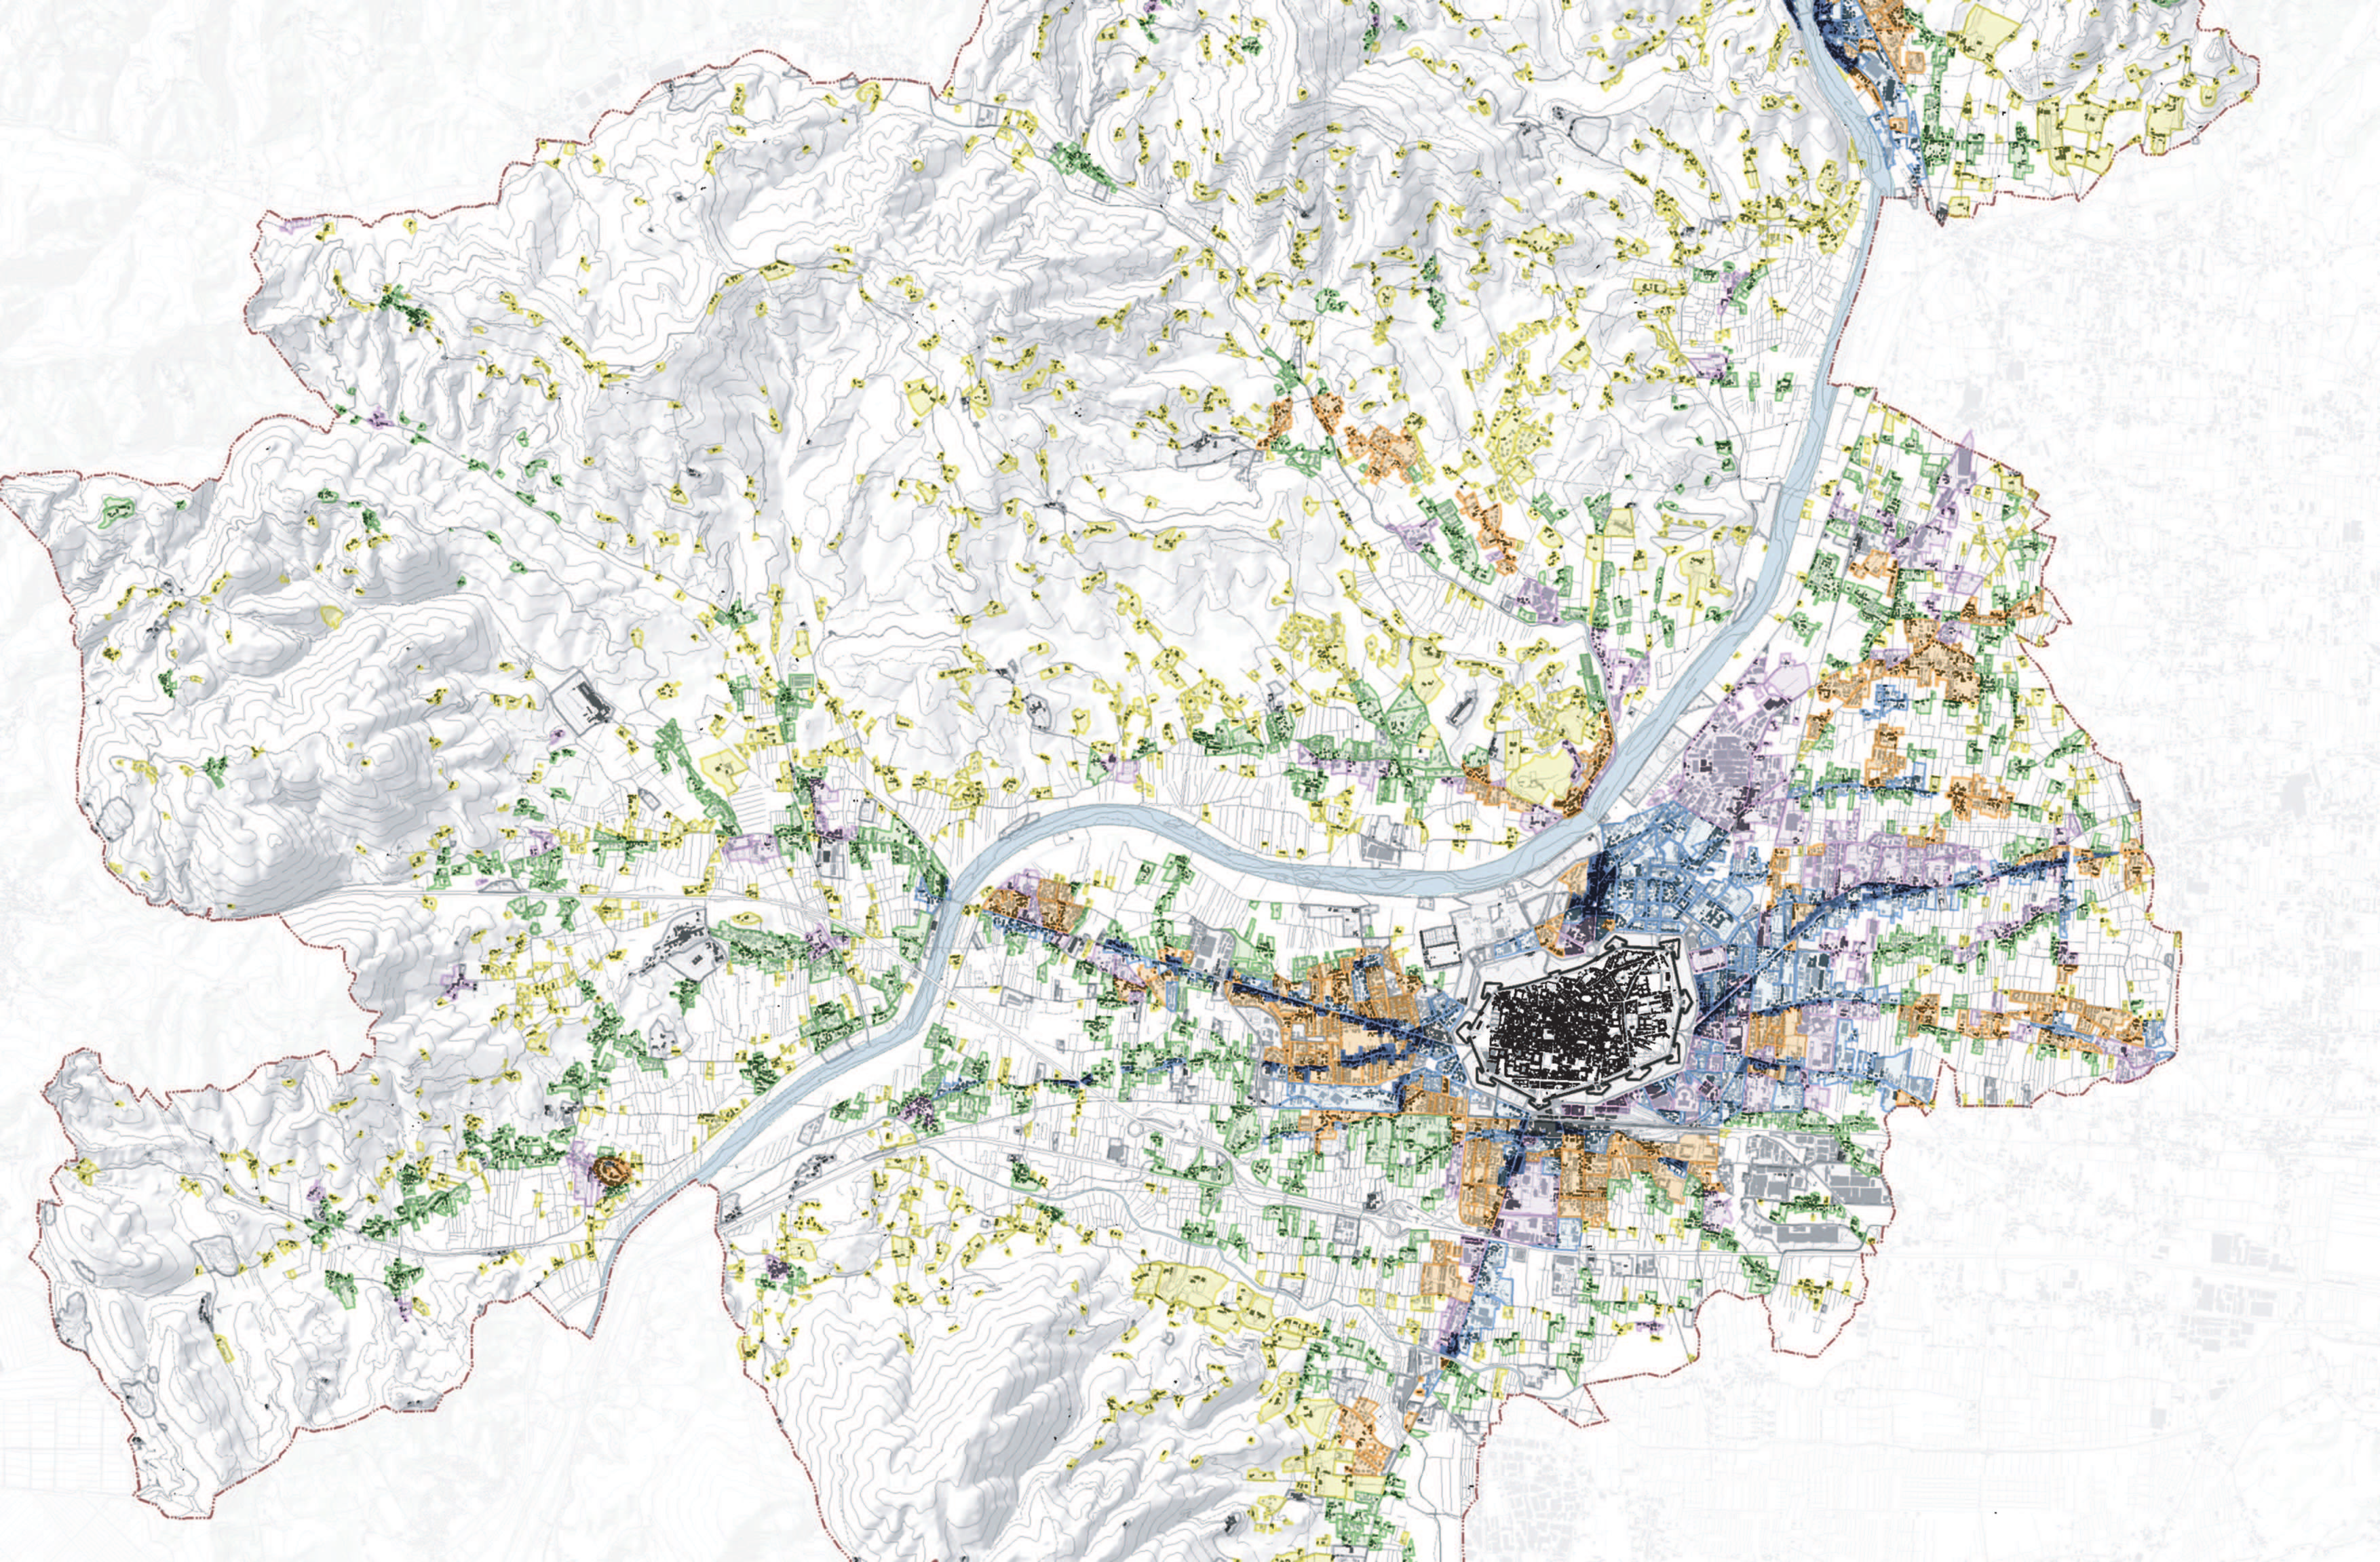
\includegraphics[width=\textwidth]{fig1.eps}}
\captionof{figure}{Urban development and the urban-rural relationship in the case of the Structural plan of Lucca, Italy. The map represents the morphological and figurative characterization of the urban fabric in the city of Lucca. In particular, it shows the development of the city toward the outside, by highlighting how the relation between the open (agricultural land) and the built environment (city) changes through the time (darker for historical settlements, lighter for newer ones) 
(Source: Author's Archive from the Research Project ``Analysis of soil consumption in the city of Lucca''). \label{Fig01}}
\end{minipage}

\begin{multicols}{2}

\vspace{\baselineskip}


\end{multicols}

\noindent
\begin{minipage}{\columnwidth}
\centering
\resizebox{\columnwidth}{!}
{\includegraphics[width=\textwidth]{fig2.eps}}
\captionof{figure}{Linkages between ecosystem services and human well-being. The strength of linkages between categories of ecosystem services and components of human well-being and indications of the extent to which it is possible for socioeconomic factors to mediate the linkage. The strength of the linkages and the potential for mediation differ in different ecosystems and regions. (Source: \citep{mr01}). \label{Fig01}}
\end{minipage}

\begin{multicols}{2}

\vspace{\baselineskip}

\section{A Growing Need for Nature in The City: Toward a Better Quality of Life and The Sustainability Transition}
\noindent The relationship between humans and the natural environment over the last century has undergone constant degradation, which is evinced in the widespread individual and social malaise. Today, reuniting humans with their environmental context in order to increase their quality of life cannot be delayed, and the landscape, intended as a ``spatial configuration laden with meaning and an irreplaceable link between humans and natural resources'', can facilitate this reconnection \citep{r12}. The connection between landscape and well-being was also recognized by the European Landscape Convention (ELC), which highlights how the landscape ``undertakes important functions of general interest on the cultural, ecological, and social planes\ldots [It] constitutes an essential aspect in the context of the life of populations\ldots [It] is an essential element of individual and social well-being'' \citep{r13}. So, ``Landscape is not only trees, shrubs and lawn, added for their aesthetic value. Rather, landscape combines landform, ecosystems and open-spaces networks that shape natural environment and sustain not only planting but all life forms, including humans'' \citep{r06, r14}. A sustainable approach to urban planning should reverse the traditional tendency to think city development opposed to nature, and consider urban and natural landscape fully integrated and strictly connected in a unique eco-system \citep{r16, r17}. Every city has its own landscape; its unique location and the deep understanding of its site-specific characteristics should be the starting point for each urban design strategy. The benefits of pursuing a sustainable balance between nature and city are considerable in different ways: ecologically, socially and economically. In fact, nature and vegetation positively influences the local microclimate extracting CO$_2$ from the air, reducing dust and urban pollutants, absorbing noise, raising local humidity by evapotranspiration, retaining rain water and, in general, reducing heat-island effects. The variety of types of green areas and environments, and the diversity of species and combination of plants, make the local habitat more attractive for different birds, insects and small animals, improving the biodiversity of the city and therefore also increasing the accessibility to nature and different experiences to people. The increasing quality of the microclimate, the creation of greener spaces and likeable views improve people’s health and quality of life, reducing urban stress and discomfort. Studies in the Netherlands demonstrate that children with good access to green open space, fewer high rise buildings and more outdoor sports facilities, are more physically active. Similarly, studies of eight European cities show that people who live in areas with abundant green open space are three times more likely to be physically active and 40\% cent less likely to be overweight or obese \citep{r17}. School children who have access to, or even sight of, the natural environment show higher levels of attention than those without these benefits \citep{r18}. Moreover, the proximity to parks, trees and quality green spaces makes living in the city more attractive which is reflected in property values.

\subsection{Environmental and Sustainability Factors and Implications on the Quality Of Life}
\noindent Quality of life is a term broadly used both by the general public and amongst policy-makers and practitioners. It is mostly used to evaluate the general well-being of individuals and societies, focused on separate dimensions of collective well-being, such as wealth and employment, quality of the built environment, physical and mental health, education, social disorganization, social belonging, and recreation and leisure \citep{r19}. Therefore, quality of life measures are based more on social indicators than just material living standards related mainly to individual or national aggregate levels of income. In a report of the EEA, \textit{Ensuring quality of life in European cities and towns}, quality of life is mainly defined as the availability of having public services, employment, shopping, transport, green open space, culture and sport facilities as well as space to live, apart from income \citep{r20}.

Undoubtedly, environmental and sustainability factors have great significance for quality of life. Illustrating this point, Brundtland's definition of sustainability, the definition of sustainable development, begins with human needs: ``Sustainable development meets the needs of the present generation without compromising the ability of future generations to meet their own needs'', and the World Commission on Environment and Development (WECD) further defines sustainable development as: ``A global process development that minimizes the use of environmental resources and reduces the impact on environmental sinks using processes that simultaneously improve economy and the quality of life''.``Sustainability is the continuation of the quality of life for generations to come including the proper distribution of quality of life between groups and with other parts of the world'' \citep{r21}. So, the very concept of sustainable development emphasizes the maintenance of natural resources and the natural environment as a prerequisite for developing any economic activity to achieve human well-being and quality of life. Economic activities are the means to utilize these resources and to release their potential value to society in order to meet human needs. A healthy environment and the wise use of natural resources are indispensable for sustainable development which provides the basis for long-term quality of life \citep{r22}.

\subsection{The Provision of Ecosystem Services}
\noindent All ecosystems are open systems powered by other ecosystems in a number of forms, energy, and information. This flow of energy characterizes the work of ecosystems, that is their capacity to provide goods and services (water and air quality, CO$_2$ absorption, soil protection, raw materials, recreational and cultural services, and so on) named \textit{ecosystem services} (ESs) \citep{r23}.

According to the EPA ecosystem services are defined as the products of ecological functions or processes that directly or indirectly contribute to quality of life (more directly to human well-being), or have the potential to do so in the future \citep{r24}. Moreover, the Millennium Ecosystem Assessment (MA) defines ecosystem services as the benefits people derive from ecosystems. These include provisioning services such as food and water; regulating services such as regulation of floods, drought, land degradation, and disease; supporting services such as soil formation and nutrient cycling; and cultural services such as recreational, spiritual, religious and other nonmaterial benefits \citep{r25}. There are several key components of human well-being, that can consistently affect a community's quality of life:

\begin{itemize}
	\item \textit{the basic material needs for a good life}, which refers to the ability to have a secure and adequate livelihood, including income and assets, enough food and water at all times, shelter, ability to have energy to keep warm and cool, and access to goods;
	\item \textit{health}, referring to the level of nourishment and freedom from disease, and access to adequate and clean drinking water and clean air. Health can also be linked to cultural services since they affect spiritual, inspirational, aesthetic, and recreational opportunities, and these in turn affect both physical and emotional states of people. Health is the most complex key component of human well-being because it can be affected by a number of varying, sometimes unpredictable, factors;
	\item \textit{good social relations}, these are expressed as the realization of aesthetic and recreational values, ability to express cultural and spiritual values, development of social capital and avoidance of tension and conflict over a declining resource base;
	\item \textit{personal security}, this represents the secure access to necessary resources, and the security from natural and human-made disasters. It is affected both by changes in provisioning services (that affect supplies of food and other goods and the likelihood of conflict over declining resources), and by changes in regulating services (that could influence the frequency and magnitude of floods, climate regulation, droughts and disease regulation);
	\item \textit{freedom of choice and action}, referring to the ability of individuals to control what happens to them and the ability to achieve their desires. It cannot be achieved without the existence of the other components of well-being and thus is influenced by changes in provisioning, regulating, or cultural services from ecosystems.
\end{itemize}

The concept of human well-being is complex and multidimensional. The linkages between quality of life and ecosystem services are even more complex. Even though some of these links are recognized, many remain poorly understood and controversial. The capacity of human communities to form satisfied societies, stable economies, and to plan for the future relies on environmental stability, availability of natural materials, and the adequate functioning of the cleansing and recycling processes of ecosystems \citep{r26}.

There is a two-way interaction between ecosystem condition and human activities: the first refers to the services that ecosystems provide to people, and the second refers to the impacts of human activities on ecosystem functioning. Human transformation of ecosystems, and subsequently of services they provide, may add up to or reduce the benefits to society, or directly affect a person's quality of life. The man-made change to ecosystem may lead to ecosystem services lost, which in long term may deeply affect the quality of life of communities, but also exceed the short term economic gains for society. Therefore an appropriate environmental management of urban area which takes into account the importance of ecosystem service in decision making processes could effectively contribute to the improvement of the quality of life of communities and human well-being (physical, social, economic, etc.).

\section{Fighting The Conflict: Planning and Designing New Relationships Between Humans and Nature}
\noindent As Botkin and Beveridge stated in 1997 ``In more than 2000 years of city planning, those who have written about cities have agreed on three points: 1) cities are centres of innovation and creativity in civilisation; 2) the more pleasant a city is the more likely it is that residents will be innovative and creative; 3) vegetation is the key to making cities pleasant'' \citep{r27}.

The desire for a new human/nature relationship, the necessity of an appropriate environmental management for a better functioning ecosystem calls into play the role of open spaces, green networks and rural areas into (and around) urban ones. The search for a new order and a greener city starts from the so-called green networks (infrastructures), in particular from agricultural practices and their relationship with urban areas (urban agriculture) \citep{r28, r29, r30}. These networks of open green spaces in, and around cities, have the potential to effectively contribute to the regeneration of degraded contexts, stimulating the upgrading of natural ecosystems and the maintenance of ecosystem services to improve the quality of the urban environment, and therefore the quality of life of its inhabitants \citep{r31}.

For example: in the United States, community green infrastructures and agricultural and rural practices in urban areas, have been greatly developed, not only for the achievement of urban and physical regeneration objectives, but also for social integration and economic development goals. Moreover, together with the most known \textit{community gardens} (which is the activity of gardening a piece of land by a group of people, utilizing either individual or shared plots on private or public land \citep{r32, r33, r34}) and \textit{retail farms} (which are retail essentially market featuring foods sold directly by farmers to consumers), there are a wide variety of different activities linked to agricultural production and fresh products in and around cities (\textit{feeding the city}, \textit{guerrilla food}, \textit{urban beekeeping}, \textit{urban agroforestry}, etc.). The real, wider framework at the basis of these programs is found in healthy food policies and correct eating habits as a way to tackle serious social illnesses such as high rates of obesity, diabetes, and cardiovascular diseases \citep{r35, r36, r37, r38, r06}. European trends differ in comparison, probably due the generally higher quality of urban areas on the one hand, and a higher quality food production on the other. Protection and conservation of peri-urban areas with agricultural uses and a demand for leisure activities linked to rural experiences have been growing in recent years and represent a stimulus for research and experimentation. For example, in Italy, the role of the Ecological Networks is being redefined. The most common approach considers Ecological Networks as an essential driver for managing new ecological balance in urban areas under transformation, by assigning essential and irreplaceable roles to rural areas. (Figure \ref{Fig03}). In a time of crisis like the present, this could lead to the development of an economic system based on the local scale, and respond to the growing need for sustainability of the urban system \citep{r39, r40}. Green networks and agriculture can therefore effectively regenerate the complexity of urban and peri-urban areas, becoming the new binder and relational matrix, between what is urban and what is open space. Understanding the meaning of this opportunity means giving way to new economies, policies for social inclusion, projects for landscape regeneration and plans for the rehabilitation of large settlement contexts \citep{r06}.

\vspace{\baselineskip}

\end{multicols}

\noindent
\begin{minipage}{\columnwidth}
\centering
\resizebox{\columnwidth}{!}
{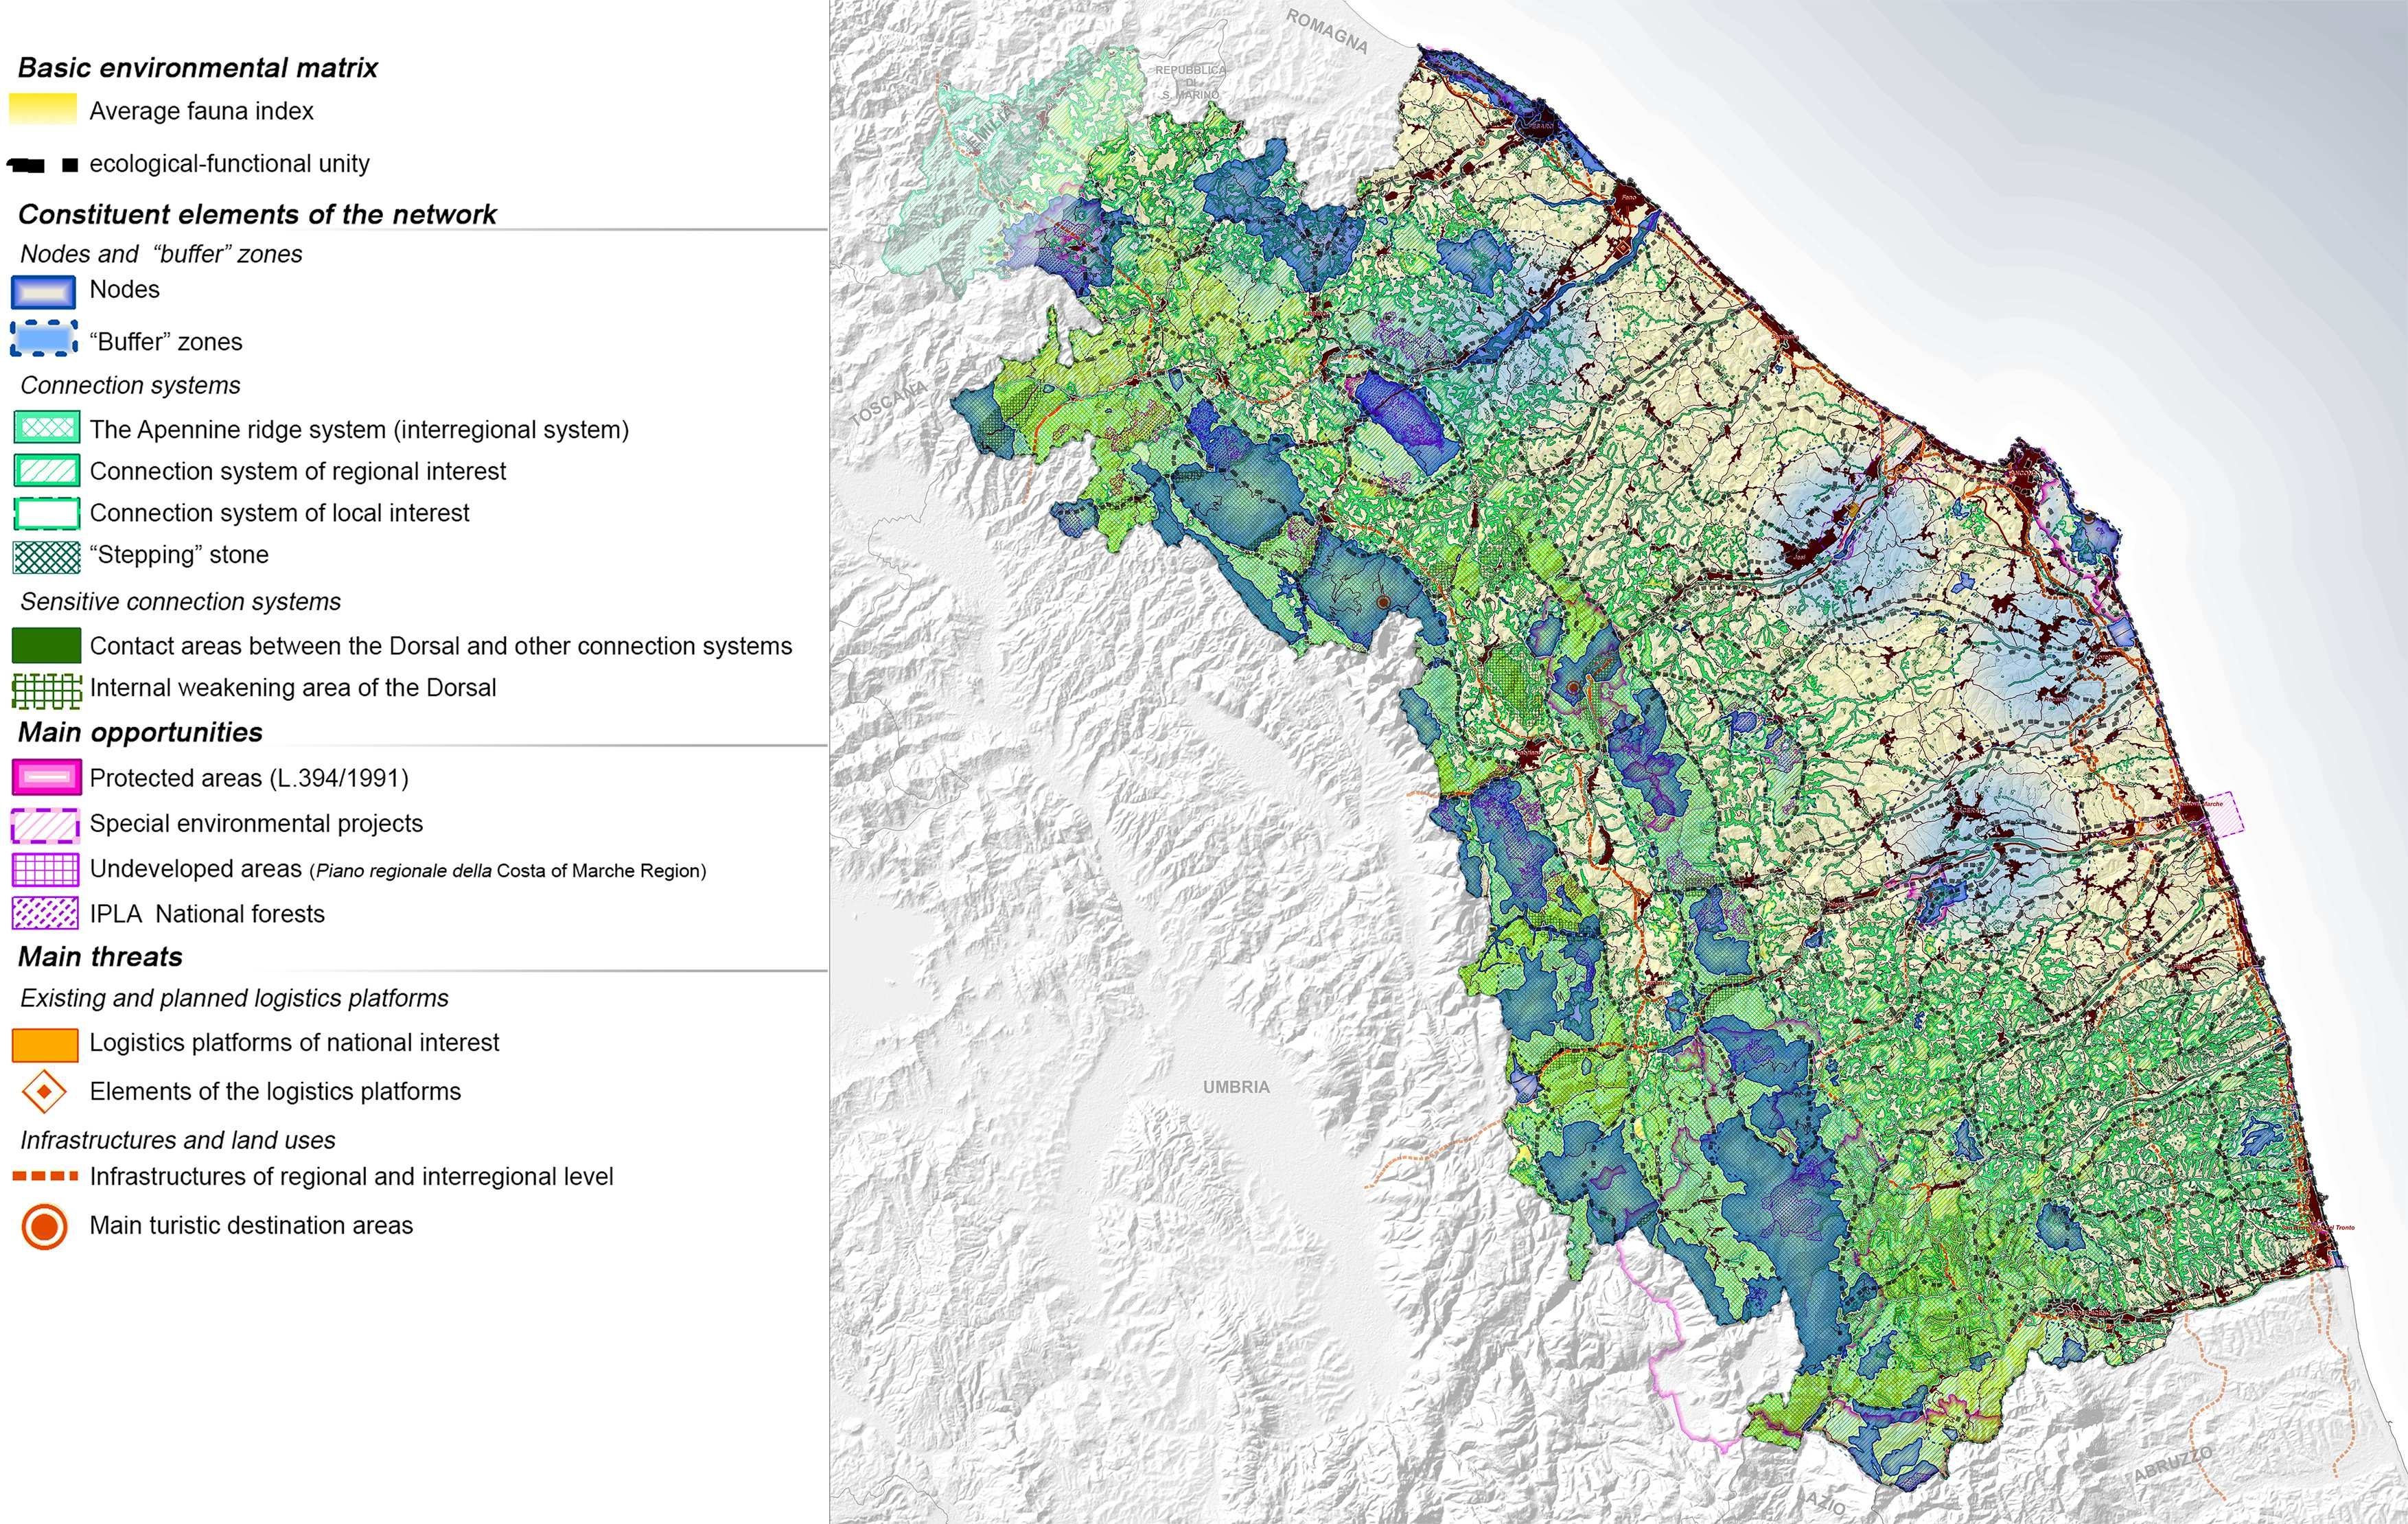
\includegraphics[width=\textwidth]{fig3.eps}}
\captionof{figure}{The case study of the ecological network of the Marche Region (REM), Italy. The map shows to Project strategy, that aims to: i) facing and planning the problem of protection and evaluation of the regional environmental heritage as a whole; ii) defining an area of intervention that concerns the entire regional territory (not just nodes and corridors), defining the forms of contact with Marche landscapes; iii) managing the regional environmental system, governing the functions of geographical and typological unity; iv) establishing modes of interaction between the REM and regional planning and programming instruments
(Source: Author's archive from the Research Project ``The Ecological Network of the Marche Region''). \label{Fig03}}
\end{minipage}

\begin{multicols}{2}

\vspace{\baselineskip}

\subsection{Green Infrastructures as Integration Process and the Real Challenge of Agriculture in and Around Cities}
\noindent The term ``green infrastructure'' was first developed by Mark Benedict and Ed McMahon (2002) of The Conservation Fund (TCF), in the early part of this century and is defined as follows: ``\textit{Green infrastructure is an interconnected network of waterways, wetlands, woodlands, wildlife habitats, and other natural areas; greenways, parks, and other conservation lands; working farms, ranches, and forests; and wilderness and other open spaces that support native species, maintain natural ecological processes, sustain air and water resources, and contribute to the health and quality of life for communities and people}" \citep{r41}.

This definition goes beyond traditional environmental planning concepts to incorporate human livability while maintaining the importance of the natural system. However, its focus on ecological processes misses a more inclusive framework to apply systematic thinking and interconnected strategies to a broader range of elements beyond ecological systems, such as cultural, social, historical, economic, and political resources, among others. Green Infrastructure is about strengthening the functionality of ecosystems for continued delivery of goods and services \citep{r42}; as well as combating biodiversity loss by increasing spatial and functional connectivity between existing natural areas and improving landscape functionality \citep{r43, r44, r45}.

The American Conservation Fund stated the following as the eight Principles of Green Infrastructure Planning, Design and Implementation \citep{r46, r47}: 1) identify and protect green infrastructure before development; 2) engage diverse people and organizations from a range of sectors; 3) linkage is key, connecting green infrastructure components with each other and with people; 4) design green infrastructure systems that function at different scales and across boundaries; 5) green infrastructure activity must be grounded in good science and planning practice; 6) fund green infrastructure up-front as a primary public investment; 7) emphasize that green infrastructure benefits are afforded to all (to nature and people); 8) green infrastructure should be the framework for conservation of natural and cultural resources. Emerges that integration, multi-scale approach and community involvement are the 'key-words' for the success of Green Infrastructure plans and project. It is also clear that Green infrastructure benefits are better achieved if green space creation and management are well integrated with more traditional land development and built infrastructure planning. But does a Green Infrastructure really consist of? With the European Green Infrastructure Strategy, the EU clarified that not all green open spaces are possible component of a Green Infrastructure, but only those of high quality and that form part of an interconnected network \citep{r48}. Examples: an urban park inside a city might be considered an integral part of Green Infrastructure if it acts as a cool air corridor, absorbs excess water run-off and offers an attractive outdoor area for recreation and wildlife; a patch of uniform grass that contains no other environmental features is unlikely to qualify as GI. In rural areas, intensively managed farmland would also not normally form part of a GI network unless it were specifically managed in a way that supports local biodiversity or that encourages a more multifunctional land use which combines food production with other benefits, like recreation or water purification \citep{r49}. This is the case of rural areas and urban agriculture, which is defined as growing, cultivating, processing, and distributing food in or around a village, town, or city \citep{r50, r51}. This simple definition however, belies the complexity of the practice. Urban agriculture lies between many issues which are seen as critical to the ongoing sustainability and livability of our urban environments: public health, healthy food access, green space, air and water quality, economic development, and community engagement \citep{r52}. Urban agriculture represents a tangible, accessible opportunity for city residents to become involved in issues of food provenance and food security and to reconnect with a food system that many feel is somehow out of their context. Additionally, urban agriculture is consistent with, and is being bolstered by, new approaches to urban design and development, which emphasize diffuse, informal, community-based initiatives, open space, green space and ``soft edge'' interventions for the overall quality and sustainability of the urban environment \citep{r53, r54, r55}. At the same time, urban areas represent a relevant experimental opportunity to stimulate innovative practices (such as multifunctional agriculture, urban gardening, and urban agri-farming) to be exploited in relation to the need to supply public services and products for the city \citep{r56}. The role of urban agriculture practices and related activities can actually be articulated on the basis of the spatial context within which they are implemented. Whether they are undertaken within small/medium towns or within large cities, their role and contribution to the social, economic and physical context is different, as is also the perception by the local population. Within large cities and metropolitan areas, urban agriculture practices are used for physical urban regeneration, land conservation, and residents leisure activities (see as examples the cases of large cities, such as Milan, London, or Paris with their plan for Green Infrastructures, Community Gardens, or Feeding the City programmes). The situation is different for small centres. The demand for "rurality" decreases with increasing potential and actual accessibility to rural areas. In such cases, their role is strictly and directly linked to the creation of opportunities for tackling decline and deprivation of the local economy (see as example, The Italian Strategy for Inner Areas, or the Community Economic Development strategy for US rural and small town). The community and neighborhood scale, therefore, plays a fundamental role in creating a sense of identity and community cohesion, which is necessary for the success of initiatives of this nature \citep{r57, r58}.

Taking the UK as an example, urban farming has a long history with urban gardening. The phenomenon of local ``allotments'' for personal farming dates back to the 1800s on national level. The multi-faceted character of urban agriculture (and the food system in general) has profound effects on many sectors, including public health, urban and land-use planning, energy, water, transport and economic development, social justice, etc. Across the country, in at least 20 cities that have experienced industrial decline, planning policies have been focused on reuse and regeneration projects for food-growing activities. As a consequence, derelict land has been substituted by green infrastructures and city farm projects \citep{r59, r60}. 

\section{Conclusion: General Strategies and Specific Planning Actions to Implement Green Infrastructures and Urban Agriculture in Local and Regional Governance}
\noindent In preceding sections we observed that redefining the relationship between agricultural areas and urban spaces can be supported by the guiding role of green infrastructures and ecosystem services.

This guiding role may come into play through:

\begin{itemize}
	\item assessing the reciprocal contamination between the landscape and ecosystem services, overcoming the physical discontinuities represented by the network and perspectives of making intersections more efficient;
	\item reassigning a potential role to decommissioned, marginalized, or abandoned spaces in the territories of settlement diffusion, which are offered to contribute to the experimentation of regenerative strategies and forms of using the city and to offer congruent local communities the opportunity for enhancement;
	\item reusing residual open spaces and abandoned places as real test banks to initiate intensive processes to reconstruct spaces for urban agriculture and to strengthen ecological networks, which develop new universes of sense for settlement models;
	\item strengthening existing ecological connections that work to order the areas awaiting new functions and which are supporting axes for the operations to transform and manage the territory;
	\item identifying players and tools to regenerate territorial capital in a view of expanding opportunities to regenerate human and social capital, developing territorial regeneration plans if necessary;
	\item rationalizing the chains that ensure the coordination of territorial intervention policies, with the aim of identifying innovative territorial planning tools capable of guaranteeing the congruence of the objectives on different scales;
	\item developing innovative means of involving local communities in constructing participatory (open-source) processes and in the demand for temporariness and reversibility of the city uses.
\end{itemize}

In order to intervene in the urban and regional governance processes with a deep commitment to success in the above points, it is necessary to integrate the large and small scales, triggering micro-changes to activate extensive processes to renew cities and territories. The use of an incremental approach able to face and manage the relationship between green infrastructures, urban agriculture and urban and territorial reorganization through ``low-intensity'' actions is also needed. This should imply low risk probabilities and not the simultaneity of large investments, allowing cross-pollination of more general, performing strategies.

This means initiating bottom-up planning in which citizens can actively contribute to pursuing ambitious objectives, such as studying effective responses to urban shrinkage and climate change, the abandonment of extended territories, and reworking collective uses of urban empty and interstitial spaces \citep{r61, r62, r06}.

The close relationship between the general strategy and actions brings into play:

\begin{itemize}
	\item relationships among the different planning scales. In this sense, it is necessary to overcome the traditional dichotomy between general planning and sectoral disciplines;
	\item relationships among directional and participatory choices. By progressively substituting the rituals of participation---with the proposals of empowerment and open-source urban planning---it is possible to give shape and substance to the constitutional principles of solidarity and subsidiarity. 
\end{itemize}

The very final result of this process is not a directional plan, but the recomposition of multiple specific urban interventions to be developed incrementally, in a continuous process of integration and contamination. In this way, it is necessary to reactivate processes of identification and consolidate the formation of either more traditional relational goods, such as the landscape or community belonging, or new ones, such as saving non-reproducible goods or the exchange economy.

\end{multicols}
\clearpage

\vspace{\baselineskip}

\begin{multicols}{2}
\renewcommand*{\refname}{\normalsize{References and Notes}}

\begin{footnotesize}
\bibliographystyle{vancouver_Librello}
\bibliography{277-Biblio}
\end{footnotesize}

\end{multicols}

\end{document}







\vspace{\baselineskip}

\noindent
\begin{minipage}{\columnwidth}
\centering
\resizebox{\columnwidth}{!}
{\includegraphics[width=\textwidth]{Fig01.jpg}}
\captionof{figure}{Community gardens in the north of Lisbon (Portugal). \label{Fig01}}
\end{minipage}




\end{multicols}
\vspace{\baselineskip}

\setlength{\tabcolsep}{3pt}
\noindent
\begin{footnotesize}
\begin{minipage}{\columnwidth}\centering
\captionof{table}{Results of a General Linear Model for the proportion of agricultural land under organic farming in French Departments (2008) as a function of plant biodiversity, landscape connectivity, proportion of Natura 2000 protected areas, latitude, longitude, altitude, human population size and department area. The number of data points is 95, the adjusted R$^2$ of the model 0.50, and the intercept 1.457 (s.e. = 2.074).}
\label{Tab01}
\begin{tabular}{lrrrrrrrr}
\toprule
 & N of plant taxa & Landscape connectivity & \% Natura 2000 & Latitude & Longitude & Altitude & Human population & Area \\
\midrule
parameter estimate & 0.264 & 0.047 & 0.113 & -0.084 & 0.003 & 0.038 & 0.056 & 0.327 \\
s.e. & 0.486 & 0.101 & 0.09 & 0.024 & 0.017 & 0.172 & 0.132 & 0.139 \\
\textit{P}-value & 0.59 & 0.64 & 0.21 &\textbf{ \textless0.001} & 0.87 & 0.82 & 0.67 & \textbf{0.02}\\
\bottomrule
\end{tabular}
\end{minipage}

\end{footnotesize}

\vspace{\baselineskip}
\begin{multicols}{2}


\begin{enumerate}[label=\alph*)]
\item
\end{enumerate}